\chapterimage{purpleLeaf.jpg} % Chapter heading image
\chapter{THE WORLD IN WHICH WE LIVE} \label{chap:01}

The world in which we live is known more to us than is the universe or, perhaps, universes in which it exists.  This world is known to be part of a solar system which is known to be part of a universe made up of similar solar systems and galaxies.  We know more about the world in which we live than we do about the universe in which it resides.  In fact, the purposes of this textbook are realized independent of knowing any more of a universal nature extant above and beyond our world.

The primary purpose of this textbook may be addressed directly by recognizing the ultimate system of interest in STEA to be \textit{the world in which we live}.  We observe the \textit{natural}, the \textit{human-made}, and the \textit{human-modified} worlds to be interconnected sectors as illustrated in \Cref{fig:humanModifiedVennDiagram}.  Of these, it is the human-modified world that should be adopted as the highest-level system of our concern, because that is where we actually live.

\begin{figure}[h]
\centering
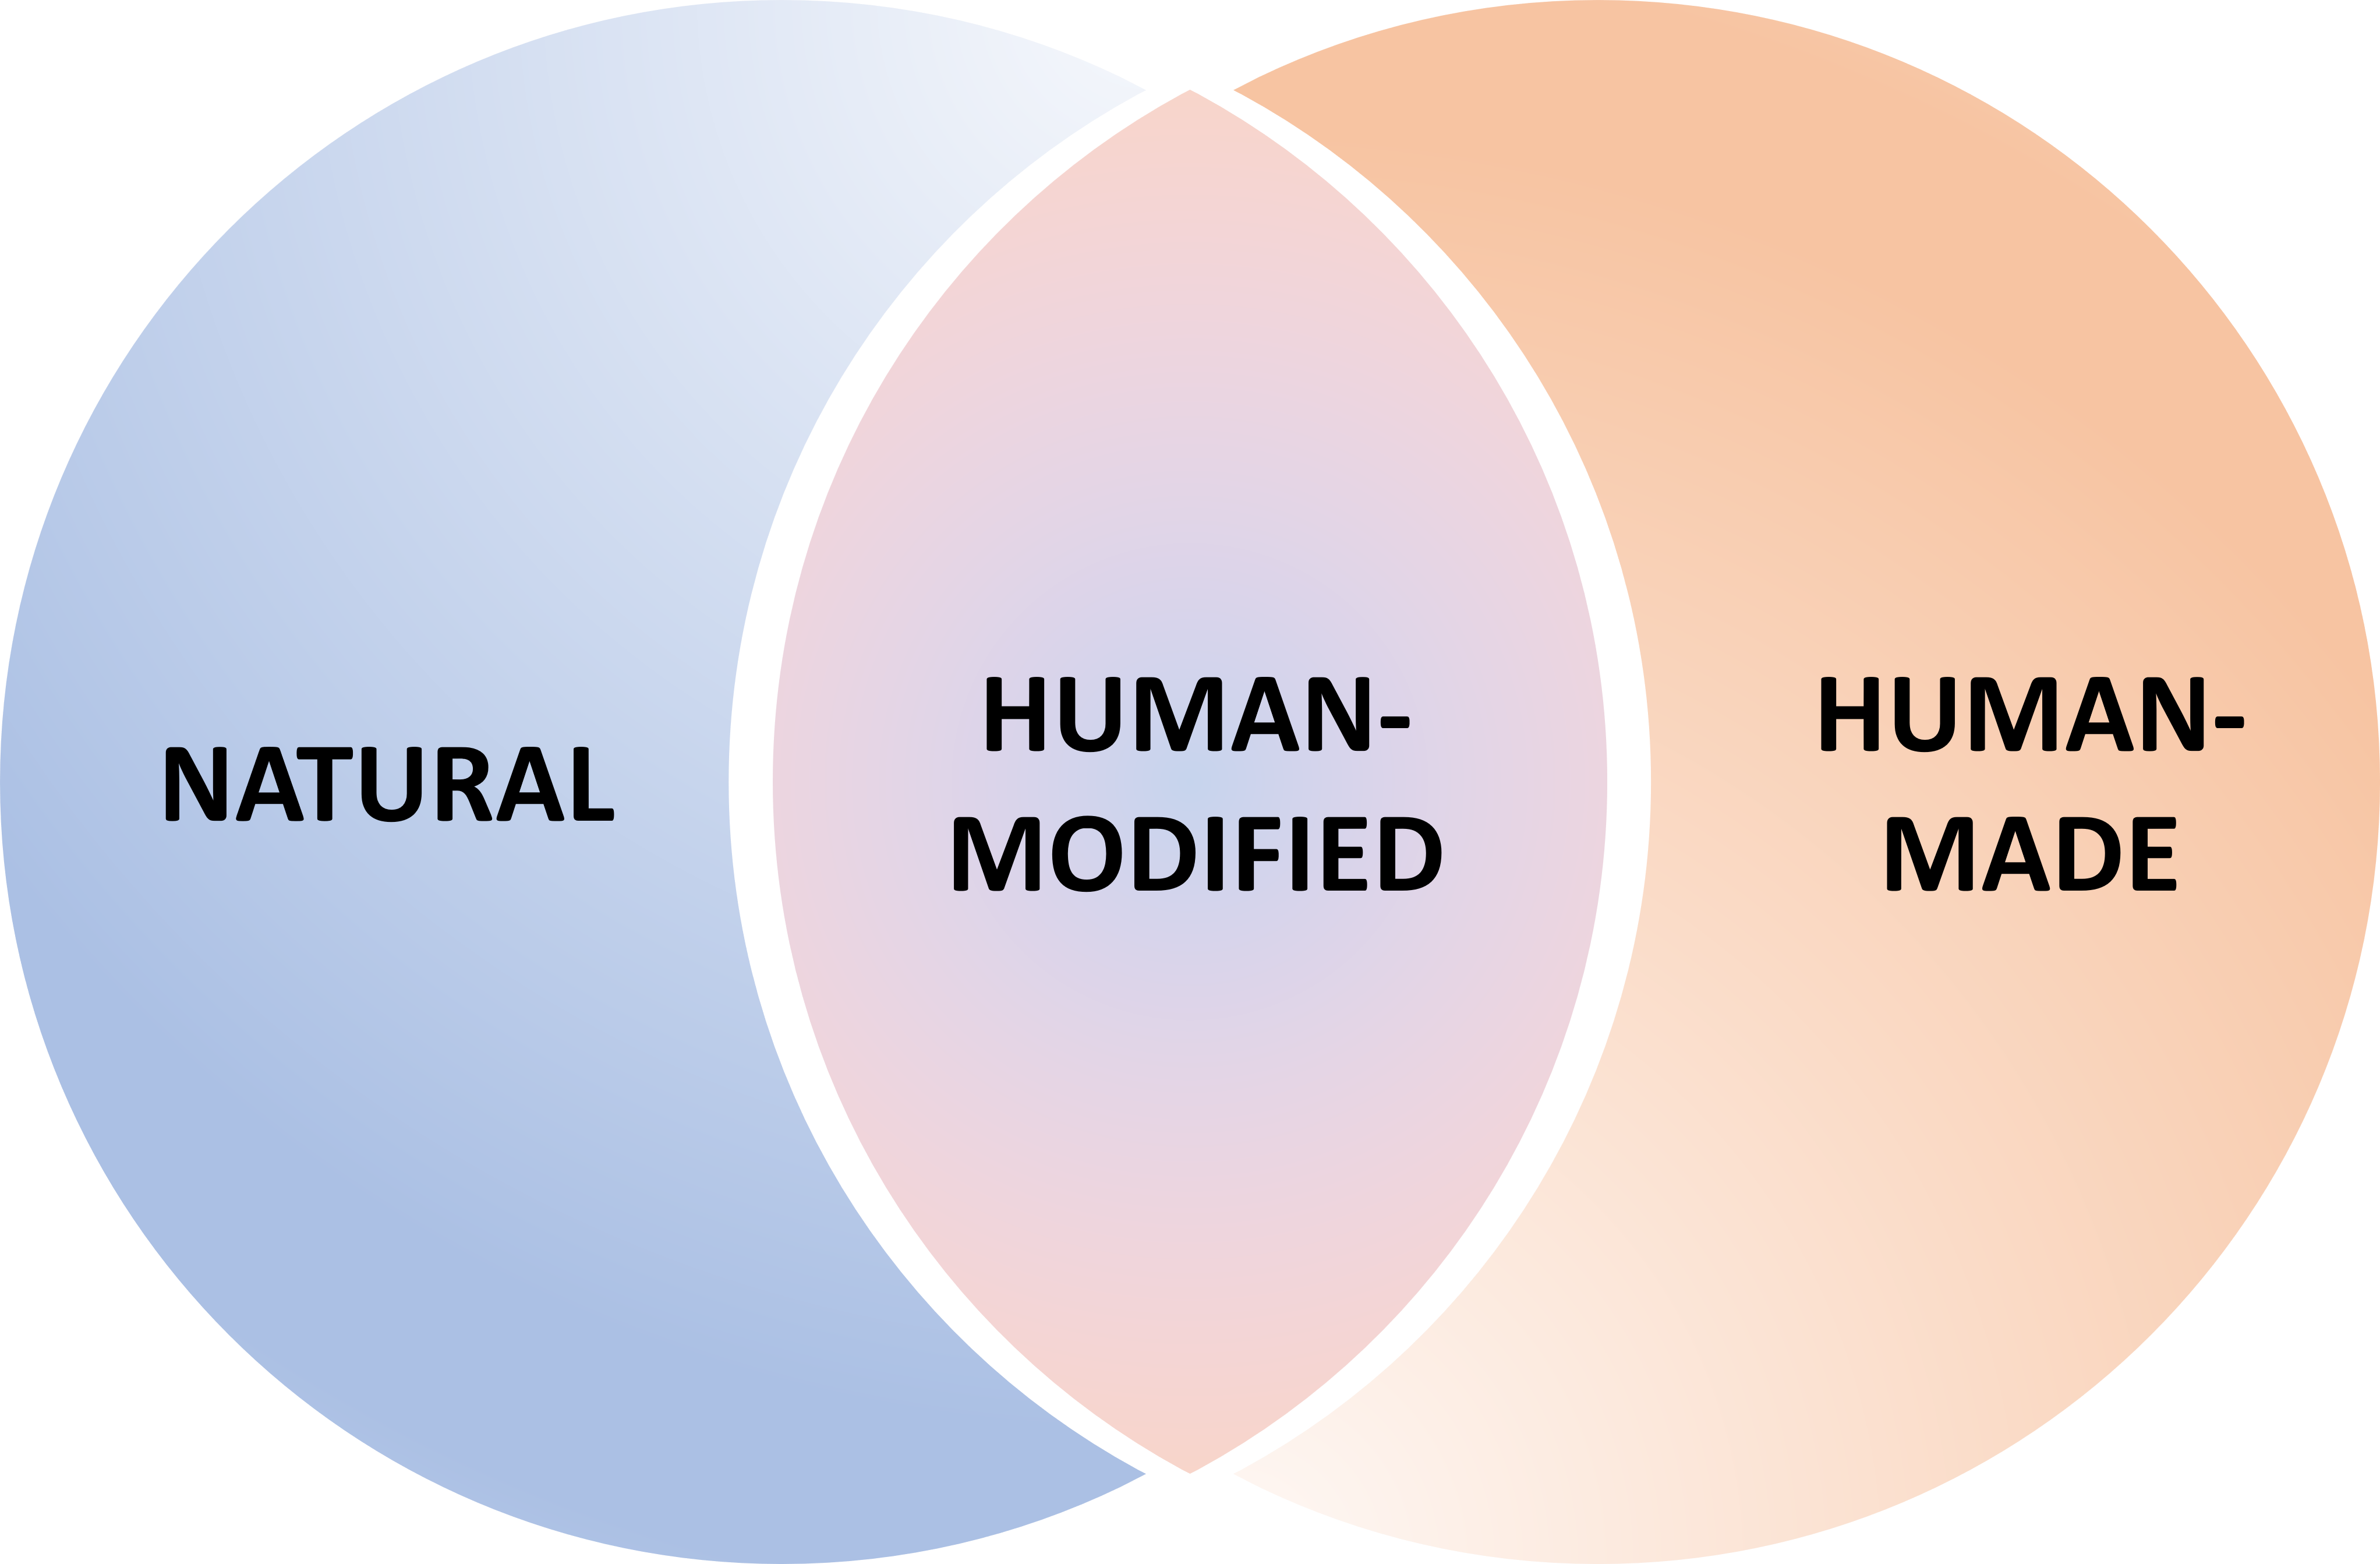
\includegraphics[width=0.9\textwidth]{humanModifiedVennDiagram.png}
\caption{Our world viewed as interconnected sectors.}
\label{fig:humanModifiedVennDiagram}
\end{figure}
    
The natural world came into being by natural processes.  The human-made world is made up of systems and products that resulted from the intervention of humans through components, attributes, and relationships.  The \textit{human-modified world} is the natural world into which the human-made has been introduced as systems, subsystems, entities, and artifacts; a world becoming increasingly complex.  This book strives to justify the human-modified world as the ultimate system level at which the viability of all that is human made should be judged.

%%----------------------------------------------------------------------------------------
%	CHAPTER CONTENT
%%----------------------------------------------------------------------------------------

\section{Sectors Comprising Our World}\index{Sectors Comprising Our World}\label{sec:sectorsComprisingWorld}

The world in which we live may be divided into the natural world and the human-made world.  Included in the former are all elements of the world that came into being by natural processes. The human-made world is made up of all human-originated systems, their product subsystems (including structures and services), and their other subsystems (such as those for production and support).  But it is the advent of the human-made that has resulted in a human-modified world as the actual world in which we live.

Systems are as pervasive as the universe in which they exist.  They are as grand as the universe itself or as infinitesimal as the atom.  This is, however, beyond the scope of STEA and requires reduction into sectors comprising our world.  Systems appeared first in natural forms, but with the advent of human beings a variety of human-made systems have come into existence.

The origin of systems gives the most important classification opportunity.  \textit{Natural systems} are those that came into being by natural processes.  \textit{Human-made systems} are those in which human beings have intervened through component, attributes, and relationships.  The \textit{human-modified system} is a natural system into which a human-made system has been integrated.

\subsection{The Natural World}\index{The Natural World}\label{sec:NaturalWorld}

The natural world is made up of all systems, including humans, that came into being by natural processes without human involvement. \textit{Natural systems} are those that came into being by natural processes. \textit{Human-made systems} are those in which human beings have intervened through components, attributes, and relationships. 

All human-made systems, when brought into being, are embedded into the natural world. Important interfaces often exist between human-made systems and natural systems. Each affects the other in some way. The effect of human-made systems on the natural world has only recently become a keen subject for study by concerned people, especially in those instances where the effect is undesirable. In some cases, this study is facilitated by analyzing the natural system as a human-modified system.

When designing a human-made system, undesirable effects can be minimized—and the natural system can sometimes be improved—by engineering the larger human-modified system instead of engineering only the human-made system. If analysis, evaluation, and validation of the human-modified system are appropriate, then the boundary of the environmental system—drawn to include the human-made system—should be considered the boundary of the human-modified system.

Natural systems exhibit a high degree of order and equilibrium. This is evidenced in the seasons, the food chain, the water cycle, and so on. Organisms and plant life adapt themselves to maintain equilibrium with the environment. Every event in nature is accompanied by an appropriate adaptation, one of the most important being that material flows are cyclic. In the natural environment there are no dead ends, no wastes, only continual re-circulation and regeneration.

Only recently have significant human-made systems appeared. These systems make up the human-made world, their chief engineer being human. The rapid evolution of human beings is not adequately understood, but their arrival has significantly affected the natural world, often in undesirable ways. Primitive beings had little impact on the natural world, for they had not yet developed potent and pervasive technologies.

An example of the impact of human-made systems on natural systems is the set of problems that arose from building the Aswan Dam on the Nile River. Construction of this massive dam ensures that the Nile will never flood again, solving an age-old problem. However, several new problems arose. The food chain was broken in the eastern Mediterranean, thereby reducing the fishing industry. Rapid erosion of the Nile Delta took place, introducing soil salinity into Upper Egypt. No longer limited by periodic dryness, the population of bilharzia (a waterborne snail parasite) has produced an epidemic of disease along the Nile. These side effects were not adequately anticipated by those responsible for the project. A system view encompassing both natural and human-made elements, as a human-modified system, might have led to a better solution to the problem of flooding. (Look for a better / more general example).


An example of the impact of human-made systems on natural systems is the set of problems that arose from building the Aswan Dam on the Nile River\footnote{\href{http://www.edc.uri.edu/temp/ci/ciip/FallClass/Docs_2006/UrbanWaterfronts/Abu-Zeid\%20and\%20El-Shibini.pdf}{Aswan Dam on the Nile}}. Construction of this massive dam ensures that the Nile will never flood again, solving an age-old problem. However, several new problems arose. The food chain was broken in the eastern Mediterranean, thereby reducing the fishing industry. Rapid erosion of the Nile Delta took place, introducing soil salinity into Upper Egypt. No longer limited by periodic dryness, the population of bilharzia (a waterborne snail parasite) has produced an epidemic of disease along the Nile. These side effects were not adequately anticipated by those responsible for the project. A system view encompassing both natural and human-made elements, as a human-modified system, might have led to a better solution to the problem of flooding.

\subsection{The Human-Made World}\index{The Human-Made World}\label{subsec:humanMadeWorld}

The human-made world is made up of all systems wherein humans have intervened through components, attributes, and relationships.

All human-made systems, when brought into being, are embedded into the natural world. Important interfaces often exist between human-made systems and natural systems. Each affects the other in some way. The effect of human-made systems on the natural world has only recently become a keen subject for study by concerned people, especially in those instances where the effect is undesirable. In some cases, this study is facilitated by analyzing the natural system as a human-modified system.

When designing a human-made system, undesirable effects can be minimized - and the natural system can sometimes be improved - by engineering the larger human-modified system instead of engineering only the human-made system. If analysis, evaluation, and validation of the human-modified system are appropriate, then the boundary of the environmental system - drawn to include the human-made system - should be considered a boundary of the human-modified system.
	
Natural systems exhibit a high degree of order and equilibrium. This is evidenced in the seasons, the food chain, the water cycle, and so on. Organisms and plant life adapt themselves to maintain equilibrium with the environment. Every event in nature is accompanied by and appropriate adaptation, one of the most important being that material flows are cyclic. In the natural environment there are no dead ends, no wastes, only continual recirculation and regeneration.

Only recently have significant human-made systems appeared. These systems make up the human-made world, their chief engineer being human. The rapid evolution of human beings is not adequately understood, but their arrival has significantly affected the natural world, often in undesirable ways. Primitive beings had little impact on the natural world, for they had not yet developed potent and pervasive technologies.

	Interesting. From a biologist’s point of view the following...
    
Anything a beaver, or even army ants, or colonial termites make is natural because it is made by a natural entity. Presumably evolution has very strongly selected for that which is made by them by eliminating many other alternatives as they arose. This ensures that at least for the near term, such innovations are fit within the environment. Until the environment changes which it usually does in the very long term.

But then why make a distinction for humans?  We have evolved also. We are natural entities. Why wouldn’t anything we make be burdened with the term “artificial” than any other thing made by a tool-using social organism?  Persons focusing only on these aspects would see the natural vs artificial controversy as empty and unnecessary.

Now, I did not make up that distinction but do use it often. All human systems including our socio-economic and socio-political institutions I consider immature artefacts. In fact, it was Nobel Laureate Herbert Simon, in whose honor NECSI grants an annual award, and whose famous book was titled, “Sciences of the Artificial” who first popularized use of the term.

Perhaps it is because scientists realize that anything man makes can be engineered so quickly that it is not subject to natural selection and evolution at first and then not even for a very long time afterward if at all. So, products that reflect more greed than adaptation to context, more arrogance than fit within natural parameters, surround our civilization. This might give some meaning to artificial. Further, the distinction might lead to a regime in which prescription and values become an important part of the process, recycling and fit in environment and cost-to-benefit an important part of the process in addition to making a buck. Len.

\subsection{Natural Versus Human-Made World}\index{Natural Versus Human-Made World}\label{subsec:naturalVsHumanWorld}

How do we classify a beaver dam?  Is it artificial or natural?  Clearly it is not designed and made by humans. This should keep the ontology folks busy.
	
To what extent is human activity not considered a part of nature? Or, do we define as synthetic anything done by the hand of man?

The universe is composed of stateful objects that undergo transformations via processes – patterns of object transformations that we as humans conceptualize in order to be able to think about cause-and-effect along the timeline.

We distinguish between natural and man-made systems (and I think they should be called by different names) because value and free will apply only to humans.

The definition of system then depends on whether it is natural or artificial.

An artificial system is an object that fulfills a function – a value-adding process from some beneficiary’s perspective.

A natural system is a collection of natural objects that are structured and behave following laws of nature.

In the discussion of “natural” vs. “man-made”, it is clear that we must decide whether to consider “man” to be a part of “nature” in the context of the discussion.

Men build dams, but we do not consider the Hoover Dam to be natural. Beavers make dams, but we deem them to be natural. Therefore, one might conclude the “we” do not consider man to be “natural” (neither man, nor his actions) in the context of the discussion. This could get downright philosophical and theological, but that is not the point.

So, are “natural” and “man-made” the words we want to use to define the concepts of “everything man DOES NOT DO” from “everything man DOES DO?”  Then, we must determine how to classify that which arises from an interaction between the two.
    
\subsection{The Human-Modified World}\index{The Human-Modified World}\label{subsec:humanModifiedWorld}

The Human-Modified World is composed of natural systems from which resources are extracted and human-made systems are embedded. We don’t live in the natural world. We don’t live in the human-made world. We live in a hybrid world at the intersection of the two already identified as the Human-Modified World. There is nothing that we do as humans that does not have one foot in the natural world and the other in the human-made world.

Since the very beginning of their existence, humans have struggled to cope with the world into which they…appeared. Knowledge, organization, and economics are the primary enablers. Human conceived existence enablers . . . 

A human-modified system is a natural system into which a human-made system has been integrated as a subsystem.

Twentieth Century man, more than his ancestors, must attempt to understand the varied peoples with whom he shares an increasingly small planet. To reach this understanding he needs to know the cultures which molded other peoples’ outlook, the history that carried them to this point.

How to select the civilizations that must be examined in a limited series of books on the history of the world’s cultures?  That is the subject of Jaques Barzun’s introduction to the Time-Life series entitled The Great ages of Man. Mr. Barzun, Dean of Faculties and Provost of Columbia University, is one of the pre-eminent cultural historians of this generation. He describes how the “revolution … in our conception of humanity” wrought by the emergence of “dozens of new peoples, new states, and new pasts” has made essential the realization that “nothing human is alien.”

In explaining the criteria for the selection of historic cultures examined in this series, he also suggests the path that present-day cultures may follow in the future.

THE EDITORS OF TIME-LIFE BOOKS (1965 Time Inc.) This book strives to justify the human-modified world as the ultimate system level at which the viability of all that is human-made should be judged. Systems thinking reveals the shortcomings of this obvious but limiting bifurcation. Consider stepping back from “The inherently presumptuous notion of human-made in favor of a continuum that starts with acceptance of the natural world as the original, or default state. Emanating from the ‘created’ state comes recognition of the advent of increasingly potent modifications by humans. The complex embedded systems that now serve humanity constitute a progressively advancing continuum between the beginning and now.”

As an example, the impact of human-made systems on natural systems is the set of problems that arose from building the Aswan Dam on the Nile River. Construction of this massive dam ensures that the Nile will never flood again, solving an age-old problem. However, several new problems arose. The food chain was broken in the eastern Mediterranean, thereby reducing the fishing industry. Rapid erosion of the Nile Delta took place, introducing soil salinity into Upper Egypt. No longer limited by periodic dryness, the population bilharzia (a waterborne snail parasite) has produced an epidemic of disease along the Nile. These side effects were not adequately anticipated by those responsible for the project. A systems view encompassing both natural and human-made elements, as a human-modified system, might have led to a better solution to the problem of flooding.

When brought into being, all that is human-made are embedded into the natural world. Important interfaces exist between human-made systems and natural systems. Each affects the other in many ways. The effect of human-made systems on the natural world has only recently become a keen subject for consideration by concerned people, especially when the effect is deemed undesirable.

Only recently have significant and complex human-made systems appeared. These systems make up the human-made world, their chief engineer being human. The rapid appearance of human beings is not adequately understood, but human presence has significantly affected the natural world, too often in undesirable ways. Primitive beings had little impact on the natural world, for they had not yet developed pervasive and potent enabling technologies.
\section{General Understanding of Systems}\index{General Understanding of Systems}\label{sec:generalUnderstandingSystems}

A system is a set of interconnected elements which form a whole and show properties which are properties of the whole rather than of the individual elements. This definition is valid for a cell, an organism, a society, or a galaxy. Joanna Macy says that a system is less a thing than a pattern – a pattern of organization. It consists of a dynamic flow of interactions which is non-summative, irreducible, and integrated at a new level of organization permitted by the interdependence of its part. The word “system” derives from the Greek “synhistanai” which means “to place together.”

From a cognitive perspective, systems thinking integrates analysis and synthesis. Natural science has been primarily reductionistic, studying the components of systems and using quantitative empirical verification. Human science, as a response to the use of a positivistic methods for studying human phenomena, has embraced more holistic approaches, studying social phenomena through qualitative means to create meaning. Systems thinking bridges these two approaches by using both analysis and synthesis to create knowledge and understanding and integrating an ethical perspective.

Analysis answers the ‘what’ and ‘how’ questions while synthesis answers the ‘why’ and ‘what for’ questions. By combining analysis and synthesis, systems thinking creates a rich inquiring platform for approaches such a social systems design, developed by Bela H. Banathy, and evolutionary systems design, as Alexander Laszlo and myself have developed to include a deeper understanding of a system in its larger context as well as a vision of the future for co-creating ethical innovations for sustainability. Just like the first image of Earth from outer space had a huge impact on our ability to see the unity of our planet, systems thinking is a way of seeing ourselves as part of larger interconnected systems.

Systems thinking is a gateway to seeing interconnections. Once we see a new reality, we cannot go back and ignore it. More importantly, that “seen” has an emotional connection, beautifully captured in the statement by Rusty Schweickart after his experience of seeing his home planet from space. – Oliver W. Holmes

What are the emotions evoked by perceiving for the first time the unity, interconnectedness, and relatedness of a system?  What are the feelings evoked by perceiving and experiencing disconnection and isolation?  Humberto Maturana says that “emotions are fundamental to what happens in all our doings” and yet, bringing up emotions in a scientific or business conversation is in many cases considered irrelevant, inappropriate or simply uncomfortable. Following Maturana’s views, I would say that the simplified answer to my two questions on the emotions evoked by unity and disconnection are love and fear, correspondingly. Love is the only emotion that expands intelligence, creativity and vision; it is the emotion that enables autonomy and responsibility. Maturana defines love as “relational behaviors through which another (a person, being, or thing) arises as a legitimate other in coexistence with oneself.”  Only in a context of safety, respect and freedom to be and create (that is, a context of love) can people be relaxed and find the conditions conductive to engage in higher intelligent behaviors that uses their brain neocortex. Learning, collaboration and creativity happen when we are able to function from a consciousness capable of including a world centric awareness of “all of us”, as Ken Wilber puts it. On the contrary, in a situation of stress, insecurity, or any other manifestation of ear, we are conditions to react more instinctually and to operate from our reptilian brain to fulfil more rudimentary needs linked to survival.

The first image of our whole Earth from space created a sense of awe and beauty. From space, we can see (and feel) its wholeness: there are no political lines dividing our national territories, there is only one whole system. However, from our terrestrial and regionally bounded experiences, we can feel that the neighbor tribe is sufficiently different and threatening to be considered an enemy.

Systems being involves embodying a new consciousness, an expanded sense of self, a recognition that we cannot survive alone, that a future that works for humanity needs also to work for other species and the planet. It involves empathy and love for the greater human family and for all our relationships – plants and animals, earth and sky, ancestors and descendants, and the many peoples and beings that inhabit our Earth. This is the wisdom of many indigenous cultures around the world, this is part of the heritage that we have forgotten, and we are in the process of recovering.

Systems being and systems living brings it all together: linking head, heart, and hands. The expression of systems being is an integration of our full human capacities. It involves rationality with reverence to the mystery of life, listening beyond words, sensing with our whole being, and expressing our authentic self in every moment of our life. The journey from systems thinking to systems being is a transformative learning process of expansion of consciousness – from awareness to embodiment.

Kathia Laszlo, Ph.D., directs Saybrook University’s program in Leadership of Sustainable Systems. This post is an excerpt from the plenary presentation “Beyond Systems Thinking: The role of beauty and love in the transformation of our world” by Dr. Kathia Laszlo at the 55th Meeting of the International Society for the Systems Sciences at the University of Hull, U.K., on July 21, 2011.

The several ways to think of and define a system include:
\begin{enumerate}
\item A system is composed of parts.
\item All the parts of a system must be related (directly or indirectly), else there are really two more distinct systems.
\item A system is encapsulated; it has a boundary.
\end{enumerate}

A system is an assemblage or combination of functionally related elements or parts forming a unitary whole, such as a river system or a transportation system. Not every set of items, facts, methods, or procedures is a system. A random group of items in a room would constitute a set with definite relationships between the items, but it would not qualify as a system because of the absence of functional relationships. This book deal primarily with systems that include physical elements and have useful purposes, including systems associated with all kinds of products, structures, and services, as well as those that consist of a coordinated body of methods or a complex scheme or plan of procedure.

\subsection{System Scope From a Boundary}\index{System Scope From a Boundary}\label{subsec:systemScopeFromBoundary}

We have said that a system has a boundary that encloses the parts of the system. Once we have set the system boundary, all of the above properties and characteristics are ``objective'', independent of human values or intentionality. But how do we reconcile this claimed objectivity with the apparent need for a human choice - presumably a subjective choice - of the system boundary?  There are two possible answers:

\begin{enumerate}
\item Some systems have a very clear physical boundary and are loosely coupled from the rest of the universe. For example, the solar system, the Earth, an airplane, and animal
\item Sometimes we are interested in a particular ``property of interest'' - the earth’s energy balance, the profitability of a business, the viability of a community, the operational effectiveness of a military system. In such cases it is usually convenient to define the boundary of the ``system of interest'' as the physical boundary of the ``system''
\end{enumerate}

Once we have established the ``property of interest'', the ``system of interest'', and corresponding system boundary can be determined by finding the set of parts and relationships that are necessary and sufficient to account for the property or properties of interest. (This I believed to be a key and novel insight – but Ashby said something similar in 1956!)

Often the system of interest and corresponding boundary will be different depending on the property of interest: for example, whether the question is ``what are we contracted to deliver'', “what is needed to achieve our purpose or goal”?  This is the difference between a ``product systems engineering'', a ``service systems engineering'', and a ``capability systems engineering'' viewpoint.

There are usually at least two boundaries we need to consider: the ``responsibility boundary'' that encloses the new or modified system (or part of a system) that we are responsible for and have control over; and the ``analysis boundary'' which includes everything else we need to consider to understand what the system of interest will actually do when deployed into the real environment.

So the key role of systems thinking as it is defined in this paper is to establish the purpose and value of the system of interest. Once the purpose and value are decided – or perhaps it is better to use the word “chosen”, because this is a human choice – the appropriate system boundary can be determined. If the wrong boundary is chosen for a system engineering effort, the wrong design choices will be made, purpose will not be achieved, and value will not be delivered. So, the skill and process for relating and aligning purpose, value and system boundary is the key to the success of a systems approach. This brings us to systems thinking.

18 century concept from the ``Encyclopedie de D. DIDEROT'':
\begin{enumerate}
\item SYSTEM (metaphysical) is nothing else than the provision of the various parts of an art or a science in a state where they support themselves all mutually, and where the last ones are explained by the first ones. Those which return reason of the others are called principles; and the system is more perfect if the principles are small in number: it is even wishing to reduce them only one. Because just as in a clock, there is a principal spring on which all the others depend, in all the systems there is also a first principle to which the various parts are subordinate to the other which make it up
\item SYSTEM (philosophy) generally means assembly or sequence of principles and conclusions; or everything and the whole of a theory of which the various parts are dependent between them, follow and depend the ones on the others
\item SYSTEM (astronomy) is the assumption of a certain arrangement of the various part which make the universe; according to this assumption the astronomers explain all the phenomena or appearances of the celestial bodies
\end{enumerate}
    
\subsection{System Descriptions and Elements}\index{System Descriptions and Elements}\label{subsec:systemDescriptionsElements}

Thus far, the search for nan acceptable system description has not ended. A valiant effort within the professional society almost ended with agreement.1 The effort was destined to be quite generic, but . . . 

Systems Function. When designing as system, the objective(s) or purpose(s) of the system must be explicitly defined and understood so that system components may be engineered to provide the desired function(s), such as a desired output for each given set of inputs. Once defined, the objective(s) or purpose(s) make possible the derivation of measures of effectiveness indicating how well the system performs. Achieving the intended purpose(s) of a human-made system and defining its measures of effectiveness are usually challenging tasks.

The purposeful action performed by a system is its function. A common system function is that of altering material, energy, or information. This alteration embraces input, process, and output. Some examples are the materials processing in a manufacturing system or a digestive system, the conversion of coal to electricity in a power plant system, and the information processing in a computer system or a customer service system.

Systems that alter material, energy, or information are composed of structural components, operating components, and flow components. Structural components are the static parts; operating components are the parts that perform the processing; and flow components are the material, energy, or information being altered. A motive force must be present to provide the alteration within the restrictions set by structural and operating components.

System components have attributes that determine the component’s contribution to the system’s function. Examples of component attributes include the color of an automobile (a characteristic), the strength of a steel beam (a quality), the number and arrangement of bridge piers (a configuration), the capacitance of an electrical circuit (a power), the maximum speed permitted by the governor of a turbine (a constraint), and whether or not a person is talking on the telephone (a state). An example of a system-level attribute is the length of runway required by an aircraft for takeoff and landing. The runway length requirement is determined by the attributes and relationships of the aircraft as a component and by the configuration attributes of the air transportation system.

A single relationship exists between two and only two components based on their attributes. The two components are directly connected in some way, though they are not necessarily physically adjacent. In a system with more than two components, at least one of the components in the relationship also has at least one relationship with some other component. Each component in a relationship provides something that the other component needs so that it can contribute to the system’s function. In order to form a relationship of maximum effectiveness, the attributes of each component must be engineered so that the collaborative functioning of the two components is optimized.

Relationships that are functionally necessary to both components may be characterized as first order. An example is symbiosis, the association of two unlike organisms for the benefit of each other. Second-order relationships, called synergistic, are those that are complementary and add to system performance. Redundancy in a system exists when duplicate components are present for the purpose of assuring continuation of the system function in case of component failure.

System Elements. Systems are composed of components, attributes, and relationships. These are described as follows:
\begin{enumerate}
\item Components are the parts of a system
\item Attributes are the properties (characteristics, configuration, qualities, powers, constraints, and state) of the components and of the system as a whole
\item Relationships between pairs of linked components are the result of engineering the attributes of both components so that the pair operates together effectively in contributing to the system’s purpose(s)
\end{enumerate}

The state is the situation (condition and location) at a point in time of the system, or of a system component, with regard to its attributes and relationships. The situation of a system may change over time in only certain ways, as in the on or off state of an electrical switching system. A connected series of changes in the state over time comprise a behavior. The set of all behaviors with their relative sequence and timing comprise the process. The process of a component may control the process of another component.

A system is a set of interrelated components functioning together toward some common objective(s) or purpose(s). The set of components meets the following requirements:
\begin{enumerate}
\item The properties and behavior of each component of the set have an effect on the properties and behavior of the set as a whole
\item The properties and behavior of each component of the set depend on the properties and behavior of at least one other component in the set
\item Each possible subset of components meets the two requirements listed above; the components cannot be divided into independent subsets
\end{enumerate}

The previous requirements ensure that the set of components constituting a system always has some property, or behavior pattern, that cannot be exhibited by any of its subsets acting alone. A system is more than the sum of its component parts. However, the components of a system may themselves be systems, and every system may be part of a larger system in a hierarchy.

When designing a system, the objective(s) or purpose(s) of the system must be explicitly defined and understood so that system components may be engineered to provide the desired function(s), such as a desired output for each given set of inputs. Once defined, the objective(s) or purpose(s) make possible the derivation of measures of effectiveness indicating how well the system performs. Achieving the intended purpose(s) of a human-made system and defining its measures of effectiveness are usually challenging tasks.

The purposeful action performed by a system is its function. A common system function is that of altering material, energy, or information. This alteration embraces input, process, and output. Some examples are the materials processing in a manufacturing system or a digestive system, the conversion of coal to electricity in a power plant system, and the information processing in a computer system or a customer service system.

Systems that alter material, energy, or information are composed of structural components, operating components, and flow components. Structural components are the static parts; operating components are the parts that perform the processing; and flow components are the material, energy, or information being altered. A motive force must be present to provide the alteration within the restriction set by structural and operating components.

System components have attributes that determine the component’s contribution to the system’s function. Example of component attributes include the color of an automobile (a characteristic), the strength of a steel beam (a quality), the number and arrangement of bridge piers (a configuration), the capacitance of an electrical circuit (a power), the maximum speed permitted by the governor of a turbine (a constraint), and whether or not a person is talking on the telephone (a state). An example of a system-level attribute is the length of runway required by an aircraft for takeoff and landing. The runway length requirement is determined by the attributes and relationships of the aircraft as a component and by the configuration attributes of the air transportation system.

A single relationship exists between two and only two components based on their attributes. The two components are directly connected in some way, though they are not necessarily physically adjacent. In a system with more than two components, at least one of the components in the relationship also has at least one relationship with some other component. Each component in a relationship provides something that the other component needs so that it can contribute to the system’s function. In order to form a relationship of maximum effectiveness, the attributes of each component must e engineered so that the collaborative functioning of the two components is optimized.

Relationships that are functionally necessary to both components may be characterized as first order. An example is symbiosis, the association of two unlike organisms for the benefit of each other. Second-order relationships, called synergistic, are those that are complementary and add to system performance. Redundancy in a system exists when duplicate components are present for the purpose of assuring continuation of the system function in case of component failure.

Systems and Subsystems. The definition of a system is not complete without consideration of its position in the hierarchy of systems. Every system is made up of components, and many components can be broken down into smaller components. If two hierarchical levels are involved in a given system, the lower is conveniently called a subsystem. For example, in an air transportation system, the aircraft, control tower, and terminals are subsystems. Equipment, people, and software are components. The designation of system, subsystem, and component are relative, because the system at one level in the hierarchy is the subsystem or component at another.

In any particular situation, it is important to define the system under consideration by specifying its limits, boundaries, or scope. Everything that remains outside the boundaries of the system is considered to be the environment. However, no system is completely isolated from its environment. Material, energy, and/or information must often pass through the boundaries as inputs to the system. In reverse, material, energy, and/or information that pass from the system to the environment are called outputs. That which enters the system in one form and leaves the system in another form is usually called throughput.

The total system, at whatever level in the hierarchy, consists of all components, attributes and relationships needed to accomplish one or more objectives. Each system has objective(s) providing purpose(s) for which all system components, attributes, and relationships have been organized. Constraints placed on the system limit its operation and define the boundary within which it is intended to operate. Similarly, the system places boundaries and constraints on its subsystems.

An example of a total system is a fire department. The subsystems of this “fire control system” are the building, the fire engines, the firefighters with personal equipment, the communication equipment, and maintenance facilities. Each of these subsystems has several contributing components. At each level in the hierarchy, the description must include all components, all attributes, and all relationships.

Systems thinking and the systems viewpoint looks at a system from the top down rather than from the bottom up. Attention is first directed to the system as a black box that interacts with its environment. Next, attention is focused on how the smaller black boxes (subsystems) combine to achieve the system objective(s). The lowest level of concern is then with individual components.

The process of bringing systems into being and of improving systems already in existence, in a holistic way, is receiving increasing attention. By bounding the total system for study purposes, the systems engineer or analyst will be more likely to obtain a satisfactory result. The focus on systems, subsystems, and components in a hierarchy forces consideration of the pertinent functional relationships. Components and attributes are important, but only to the end that the purpose of the whole system is achieved through the functional relationships linking them.

\subsection{Classification of Systems}\index{Classification of Systems}

Beyond the classification of systems that emanates from the partitioning of our world into N. HM and HJMod, are classifications of a subordinate nature. Systems may be classified for convenience and to provide insight into their wide range. In this section, classification will be accomplished by several dichotomies conceptually contrasting system similarities and dissimilarities. Descriptions are given of physical and conceptual systems, static and dynamic systems, and closed and open systems.

Physical and Conceptual Systems. Physical systems are those that manifest themselves in physical form. They are composed of real components and may be contrasted with conceptual systems, where symbols represent the attributes of components. Ideas, plans, concepts, and hypotheses are examples of conceptual systems.

A physical system consumes physical space, whereas conceptual systems are organizations of ideas. One type of conceptual system is the set of plans and specifications for a physical system before it is actually brought into being. A proposed physical system may be simulated in the abstract by a mathematical or another conceptual model. Conceptual systems often play an essential role in the operation of physical systems in the real world.

The totality of elements encompassed by all components, attributes, and relationships focused on a given result employ a process that determines the state changes (behaviors) of a system. A process may be mental (thinking, planning, and learning), mental-motor (writing, drawing, and testing), or mechanical (operating, functioning, and producing). Processes exist in both physical and conceptual systems.

Process occurs at many different levels within systems. The subordinate process essential for the operation of a total system is provided by the subsystem. The subsystem may, in turn, depend on more detailed subsystems. System complexity is the feature that defines the number of subsystems present and, consequently, the number of processes involved. A system may be bounded for the purpose of study at any process or subsystem level. Also, related systems that are normally analyzed individually may be studied as a group, and the group is often called a system-of-systems (SOS).

Static and Dynamic Systems.  Another system dichotomy is the distinction of static and dynamic types. A static system is one whose states do not change because it has structural components but no operating or flow components, as exemplified by a bridge. A dynamic system exhibits behaviors because it combines structural components with operating and/or flow components. An example is a school, combining a building, students, teachers, books, curricula, and knowledge.

A dynamic conception of the universe has become a necessity. Yet, a general definition of a system as an ongoing process is incomplete. Many systems would not be included under this broad definition because they lack operating and flow components. A highway system is static, yet it contains the system of elements of components, attributes, and functional relationships.

A system is static only in a limited frame of reference. A bridge system is constructed, maintained, and altered over a period of time. This is a dynamic process conducted by a construction subsystem operating on a flow of construction materials. A structural engineer must view the bridge’s members as operating components that expand and contract as they experience temperature changes.

A static system serves a useful purpose only as a component or subsystem of a dynamic system. For example, a static bridge is part of a dynamic system with an overpass operating component processing a traffic flow component and with an underpass component handling water or traffic flow.

Systems may be characterized as having random properties. In almost all systems in both the natural and human-made categories, the inputs, process, and output can only be described in statistical terms. Uncertainty often occurs in both the number of inputs and the distribution of these inputs over time. For example, it is difficult to predict exactly the number of passengers who will check in for a flight, or the exact time each will arrive at the airport. However, because these factors can be described in terms of probability distributions, system operation may be considered probabilistic in its behavior.

For centuries, humans viewed the universe of phenomena as immutable and unchanging. People habitually thought in terms of certainties and constants. The substitution of a process-oriented description for the static description of the universe, and the idea that almost anything can be improved, distinguishes modern science and engineering from earlier thinking.

Closed and Open Systems. A closed system is one that does not interact significantly with its environment. The environment provides only a context for the system. Closed systems usually exhibit the characteristic of equilibrium resulting from internal rigidity that maintains the system in spide of influences from the environment. An example is the chemical equilibrium eventually reached in a closed vessel when various reactants are mixed together, provided that the reaction does not increase pressure to the point that the vessel explodes. The reaction and pressure can be predicted from a set of initial conditions. Closed systems involve deterministic interactions, with a one-to-one correspondence between initial and final states. There are relatively few closed systems in the natural and the human-made world.

An open system allows information, energy, and matter to cross its boundaries. Open systems interact with their environment, examples being plants, ecological systems, and business organizations. They exhibit the characteristics of steady state, wherein a dynamic interaction of system elements adjusts to changes in the environment. Because of this steady state, open systems are self-regulatory and often self-adaptive.

It is not always easy to classify a system as either open or closed. Open systems are typical of those that have come into being by natural processes. Human-made systems have both open and closed characteristics. They may reproduce natural conditions not manageable in the natural world. They are closed when designed for invariant input and statistically predictable output, as in the case of a spacecraft in flight.
Both closed and open systems exhibit the property of entropy. Entropy is defined here as the degree of disorganization in a system and is analogous to the use of the term in thermodynamics. In the thermodynamic usage, entropy is the energy unavailable for work resulting from energy transformation from one form to another.

In systems, increased entropy means increased disorganization. A decrease in entropy occurs as order occurs. Life represents a transition from disorder to order. Atoms of carbon, hydrogen, oxygen, and other elements become arranged in a complex and orderly fashion to produce a living organism. A conscious decrease in entropy must occur to create a human-made system. All human0made systems, from the most primitive to the most complex, consume entropy because they involve the creation of more orderly states from less orderly states.

Scientific System Classifications. Science systems and the application of science systems thinking has been grouped into three categories based on the techniques used to tackle a system:
\begin{enumerate}
\item Hard systems – involving simulations, often using computers and the techniques of operation research/management science. Useful for problems that can justifiably be quantified. However, it cannot easily consider unquantifiable variables (opinions, culture, politics, etc.), and may treat people as being passive, rather than having complex motivations
\item Soft systems – For systems that cannot easily be quantified, especially those involving people holding multiple and conflicting frames of reference. Useful for understanding motivations, viewpoints, and interactions and addressing qualitative as well as quantitative dimensions of problem situations. Soft systems are a field that utilizes foundation methodological work developed by Peter Checkland, Brian Wilson and their colleagues at Lancaster University Morphological analysis is a complementary method for structuring and analyzing non-quantifiable problem complexes
\item Evolutionary systems – Bela H. Banathy developed a methodology that is applicable to the design of complex social systems. This technique integrates critical systems inquiry with soft systems methodology. Evolutionary systems, like dynamic systems are understood as open, complex systems, but with the capacity to evolve over time. Banathy uniquely integrated the interdisciplinary perspectives of systems research (including chaos, complexity, cybernetics), cultural anthropology, evolutionary theory, and others
\end{enumerate}

The systems thinking approach incorporates several tenets:
\begin{enumerate}
\item Interdependence of objects and their attributes – independent elements can never constitute a system.
\item Holism – emergent properties not possible to detect by analysis should be possible to define by a holistic approach.
\item Goal seeking – systemic interaction must result in some goal or final state.
\item Inputs and Outputs – in a closed system inputs are determined once and constant; in an open system additional inputs are admitted from the environment.
\item Transformation of inputs into outputs – this is the process by which the goals are obtained.
\item Entropy – the amount of disorder or randomness present in any system.
\item Regulation – a method of feedback is necessary for the system to operate predictably.
\item Hierarchy – complex wholes are made up of smaller subsystems.
\item Differentiation – specialized units perform specialized functions.
\item Equifinality – alternative ways of attaining the same objectives (convergence).
\item Multifinality – attaining alternative objectives from the same inputs (divergence).
\end{enumerate}

A treatise on systems thinking ought to address many issues including:

\begin{enumerate}
\item Encapsulation of a system in space and/or time
\item Active and passive systems (or structures)
\item Transformation by an activity system of inputs into outputs
\item Persistent and transient systems
\item Evolution, the effects of time passing, the life histories of systems and their parts.
\item Design and designers.
\end{enumerate}
\section{Technology and Engineered Systems}\index{Technology and Engineered Systems}

Technology is broadly defined as the branch of knowledge that deals with the mechanical and industrial arts, applied science, and the engineering, or the sum of the ways in which social groups provide themselves with the material objects and the services of their civilization. A key attribute of a civilization is the inherent ability and the knowledge to maintain its store of technology. Modern civilizations possess pervasive and potent technology that makes possible needed systems manifested as products, which include structures and services.

\subsection{Technical Systems}\index{Technical Systems}

Science and technology is a phrase used often. Translated into its systems counterpart, this phrase prompts consideration of the link between systems science and technical systems. Technical or engineered systems have their foundation in both the natural and the systems sciences. They are a prominent and pervasive sector of the human-made world.

The phrase technical system may be used to represent all types of human-made artifacts, including technical products and processes. Accordingly, the technical system is the subject of the collection of activities that are performed by engineers within the processes of engineering design, including generating, retrieving, processing, and transmitting product information. It is also the subject of production processes, including work preparation and planning. It is also the subject of many economic considerations, both within enterprises and society.

In museums, thousands of technical objects are on display, and they are recognized as products of technology. Their variety of functions, form, size, and so forth tends to obscure common properties and features. But vast variety also exists in nature, and in those circumstances clearly defined kingdoms of natural objects have been defined for study in the natural sciences. Likewise, attempts have been made to define terms that conceptually describe classes of technical objects.

Technical objects can be referred to simply as objects, entities, things, machines, implements, products, documents, or technical works. The results of a manufacturing activity, as the conceptual content of technology, can be termed artifacts or instrumentum. Such definitions are meant to include all manner of machines, appliances, implements, structures, weapons, and vessels that represent the technical means by which humans achieve their ends. But, to be complete, this definition must recognize the hierarchical nature of systems and the interactions that occur between levels in the hierarchy. For example, the ``system'' of interest may be a transportation system, an airline system within the transportation system, or an aircraft system contained within the airline system.

Little difficulty exists in the classification of systems as either natural, technical (human-made), or human-modified. But it is difficult to classify technical systems accurately. One approach is to classify in accordance with the well-established subdivisions of technology in industry, for example, civil engineering, electrical engineering, and mechanical engineering. However, from a practical and organizational viewpoint, this does not permit a precise definition of a mechanical system or electrical system because no firm boundary can be established by describing these systems as outcomes of mechanical or electrical engineering.

Modern developments of technical systems have generally blurred the boundaries. Electronic and computer products, especially software, are increasingly used together with mechanical and human interfaces. Each acts as a subsystem to a system of greater complexity and purpose. Most systems in use today are hybrids of the simple systems of the past.

\subsection{Technological Growth and Change}\index{Technological Growth and Change}

Technological growth and change is occurring continuously and is initiated by attempts to respond to unmet deficiencies and by attempts to perform ongoing activities in a more effective and efficient manner. In addition, changes are being stimulated by political objectives, social factors, and ecological concerns.

As examples, environmental concerns have resulted in recent legislation and regulations requiring new methods for crop protection from insects, new means for the disposal of medical waste, and new methods for treating solid waste. Concern for shortages of fossil fuel sources as well as ecological impacts brought about a great focus on energy conservation and alternative energy sources. These and other comparable situations were created through both properly planned programs and as a result of panic situations. A common outcome is that all have stimulated beneficial technological innovation.

The world is increasing in complexity because of human intervention. Through the advent of advanced technologies, transportation times have been greatly reduced, and vastly more efficient means of communication have been introduced. Every aspect of human existence has become more intimate and interactive. The need for integration of ideas and conflict resolution becomes more important. At the same time, increasing populations and the desire for larger and better systems is leading to the accelerated exploitation of resources and increased environmental impact. A variety of technically literate specialists, if properly organized and incentivized, can meet most needs that arise from technological advancement and change.

Technology and Society. Human society is characterized by its culture. Each human culture manifests itself through the media of technology. In turn, the manifestation of culture is an important indicator of the degree to which a society is technologically advanced

The entire history of humankind is closely related to the progress of technology. But, technological progress is often stressful on people and their cultures alike. This need not be. The challenge should be to find ways for humans to live better lives as a result of new technological capability and social organization structure.

In general, the complexity of systems desired by societies is increasing. As new technologies become available, the pull of ``want'' is augmented by a push to incorporate these new capabilities into both new and existing systems. The desire for better systems produces an ever-changing set of requirements. The identification of the ``true'' need in answer to a problem and the elicitation of ``real'' requirements is, in itself, a technological challenge.

Transition from the past to present and future technological states is not a one-step process. Continuing technical advances become available to society as time unfolds. Societal response is often to make one transition and then to adopt a static pattern of behavior. A better response would be to seek new and well-thought-out possibilities for continuous advancement. Improvement in technological literacy should increase the population of individuals capable of participating in this desirable activity. One key to imparting this literacy is the communication technologies now expanding at a rapid pace. Thus, technology in this sphere may act favorably to aid the understanding and subsequent evaluation by society of technologies in other spheres.
\section{Transitioning Into the Systems Age}\index{Transitioning Into the Systems Age}

Evidence suggests that the advanced nations of the world are leaving one technological age and entering another. It appears that this transition is bringing about a change in the conception of the world in which we live. This conception is both a realization of the complexity of natural and human-made systems and a basis for improvement in humankind’s management of these systems. Long-term sustainability of both human-made systems and the natural world is becoming a common desideratum.

Transition to the Systems Age spawned the systems sciences and, driven by potent technologies, established a compelling need for systems engineering. Accordingly, selected definitions of systems engineering are given at the end of this chapter. Many others exist, but are not included herein. However, in conformity with the theme of this textbook, systems engineering may be described as a technologically-based interdisciplinary process for bringing systems into being. Systems engineering is an engineering interdisciplines in its own right, with important engineering domain manifestations.

\subsection{The Machine Age}\index{The Machine Age}

Two ideas have been dominant in the way people seek to understand the world in which we live. The first is called reductionism. It consists of the belief that everything can be reduced, decomposed, or disassembled to simple indivisible parts. These were taken to be atoms in physics; simple substances in chemistry; cells in biology; and monad, instincts, drives, motives, and needs in psychology.

Reductionism gives rise to an analytical way of thinking about the world, a way of seeking explanations and understanding. Analysis consists, first, of taking apart what is to be explained, disassembling it, if possible, down to the independent and indivisible parts of which it is composed; second, of explaining the behavior of these parts; and, finally, of aggregating these partial explanations into an explanation of the whole. For example, the analysis of a problem consists of breaking it down into a set of as simple problems as possible, solving each, and assembling their solutions into a solution of the whole. If the analyst succeeds in decomposing a problem into simpler problems that are independent of each other, aggregating the partial solutions is not required because the solution to the whole is simply the sum of the solutions to its independent parts. In the industrial or Machine Age, understanding the world was taken to be the sum, or result, of an understanding of its parts, which were conceptualized as independently of each other as was possible.

The second basic idea was that of mechanism. All phenomena were believed to be explainable by using only one ultimately simple relation, cause and effect. One thing or event was taken to be the cause of another (its effect) if it was both necessary and sufficient for the other. Because a cause was taken to be sufficient for its effect, nothing was required to explain the effect other than the cause. Consequently, the search for causes was environment free. It employed what is not called ``closed-system'' thinking. Laws such as that of freely falling bodies were formulated so as to exclude environmental effects. Specially designed environments, called laboratories, were used so as to exclude environmental effects on phenomena under study. Causal-based laws permit no exception. Effects are completely determined by causes. Hence, the prevailing view of the world was deterministic. It was also mechanistic because science found no need for teleological concepts (such as functions, goals, purposes, choice, and free will) in explaining any natural phenomenon. They considered such concepts to be unnecessary, illusory, or meaningless. The commitment to causal thinking yielded a conception of the world as a machine; it was taken to be like a hermetically sealed clock - a self-contained mechanism whose behavior was completely determined by its own structure.

The Industrial Revolution brought about mechanization, the substitution of machines for people as a source of physical work. This process affected the nature of work left for people to do. They no longer did all the things necessary to make a product; they repeatedly performed a simple operation in the production process. Consequently, the more machines were used as a substitute for people at work, the more workers were made to behave like machines. The dehumanization of work was an irony of the Industrial Revolution and Machine Age.

\subsection{The Systems Age}\index{The Systems Age}

Although eras do not have precise beginnings and endings, the 1940s can be said to have contained the beginning of the end of the Machine Age and the beginning of the Systems Age. This new age is the result of a new intellectual framework in which the doctrines of reductionism and mechanism and the analytical mode of thought are being supplemented by the doctrines of expansionism, teleology, and a new synthetic (or systems) mode of thought.

Expansionism is a doctrine that considers all objects and events, and all experiences of them, as parts of larger wholes. It does not deny that they have parts, but it focuses on the wholes of which they are part. It provides another way of viewing things, in a way that is different from, but compatible with, reductionism. It turns attention from ultimate elements to a whole with unrelated parts - to systems.

Preoccupation with systems brings with it the synthetic mode of thought. In the analytic mode, an explanation of the whole was derived from explanations of its parts. In synthetic thinking, something to be explained is viewed as part of a larger system and is explained in terms of its role in that larger system. The Systems Age is more interested in putting things together than in taking them apart.

Analytic thinking is outside-in thinking; synthetic thinking is inside-out thinking. Neither negates the value of the other, but by synthetic thinking on can gain understanding that cannot be obtained through analysis, particularly of collective phenomena.

The synthetic mode of thought, when applied to systems problems, is called systems thinking or the systems approach. This approach is based on the observation that when each part of a system performs as well as possible, the system as a whole may not perform as well as possible. This follows from the fact that the sum of the functioning of the parts is seldom equal to the functioning of the whole. Accordingly, the synthetic mode seeks to overcome the often observed predisposition to perfect details and ignore system outcomes.

Because the Systems Age is teleologically oriented, it is preoccupied with systems that are goal seeking or purposeful; that is, systems that offer the choice of either means or ends, or both. It is interested in purely mechanical systems only insofar as they can be used as enablers for purposeful systems. Furthermore, the Systems Age is largely concerned with purposeful systems, some of whose parts are purposeful; in the human domain, these are called social groups. The most important class of social groups is the one containing systems whose parts perform different functions that have a division of functional labor; these are called organizations.

In the Systems Age, attention in focused on groups and on organizations as parts of larger purposeful societal systems. Participantive management, collaboration, group decision making, and total quality management are new working arrangements within the organization. Among organizations is now found a keen concern for social and environmental factors, with economic competition continuing to increase worldwide.
\section{The Evolution of Systems Thinking}\index{The Evolution of Systems Thinking}

Systems thinking is subjective. It is the cognitive and cognation process of seeking understanding about the interactive influences of entities within a whole. Thinking about the engineering of systems, as presented here, encompasses entities and wholes within the context of our existence.

But systems thinking is not pervasive enough, nor is it adequately comprehensive. 

\begin{enumerate}
\item The boundary of a system is a decision made by an observer, or a group of observers.
\item A system can be nested inside another system.
\item A system can overlap with another system.
\item A system is bounded in time.
\item A system is bounded in space, though the parts are not necessarily co-located.
\item A system receives input from, and sends output into, the wider environment.
\item Science systems thinkers consider that:
\item A system is a dynamic and complex whole, interacting with a structured functional unit. Energy, material, and information flow among the different elements that compose the system;
\item A system is a community situated within an environment. Energy, material, and information flow from and to the surrounding environment via semi-permeable membranes or boundaries;
\item Systems are often composed of entities seeking equilibrium but can exhibit oscillating, chaotic, or exponential behavior.
\end{enumerate}

A holistic system is any set (group) of interdependent or temporally interacting parts. Parts are generally systems themselves and are composed of other parts, just as systems are generally parts or halons of other systems.

Two parts to be considered: 1) the desired human-made system and, 2) the engineering of that system. Both are within the goal of focused systems thinking on the well-being of humans that exist within the human-modified world; that is, the world emerging from the natural world through purposeful design by humans.

\subsection{World Focused Systems Thinking}\index{World Focused Systems Thinking}

World focused systems thinking starts with the premise that “systems science” exists, or at least a “theory of systems” is available to define systems and system properties. These properties of a system – which can be either natural or human-made, and which can exhibit a greater or lesser degree of adaptive behavior – are independent of how and why it was created. The nature of such systems is independent of human intentionality, and we see similar or identical system properties and patterns recurring across different domains of application.

Systems thinking is the process of understanding how things influence one another within a whole. In nature, systems thinking examples include ecosystems in which various elements such as air, water, movement, plants, and animals work together to survive or perish. In organizations, systems consist of people, structures, and processes that work together to make an organization healthy or unhealthy. In economics …

World focused systems thinking seems to be a stretch. But, it is necessary as the basis for looking beyond the world in which we live. This is for completeness within the scope of what is known by humans currently.

Consider Figure 1.2. Depicted is a view beyond the world in which we live. This is deemed necessary to acknowledge the universe of which our world is a part. We know little about that universe and others being mentioned. And, there is no attempt in this book to reach that far in bringing the human-made into being. Maybe someday!

\begin{figure}[h]
\centering
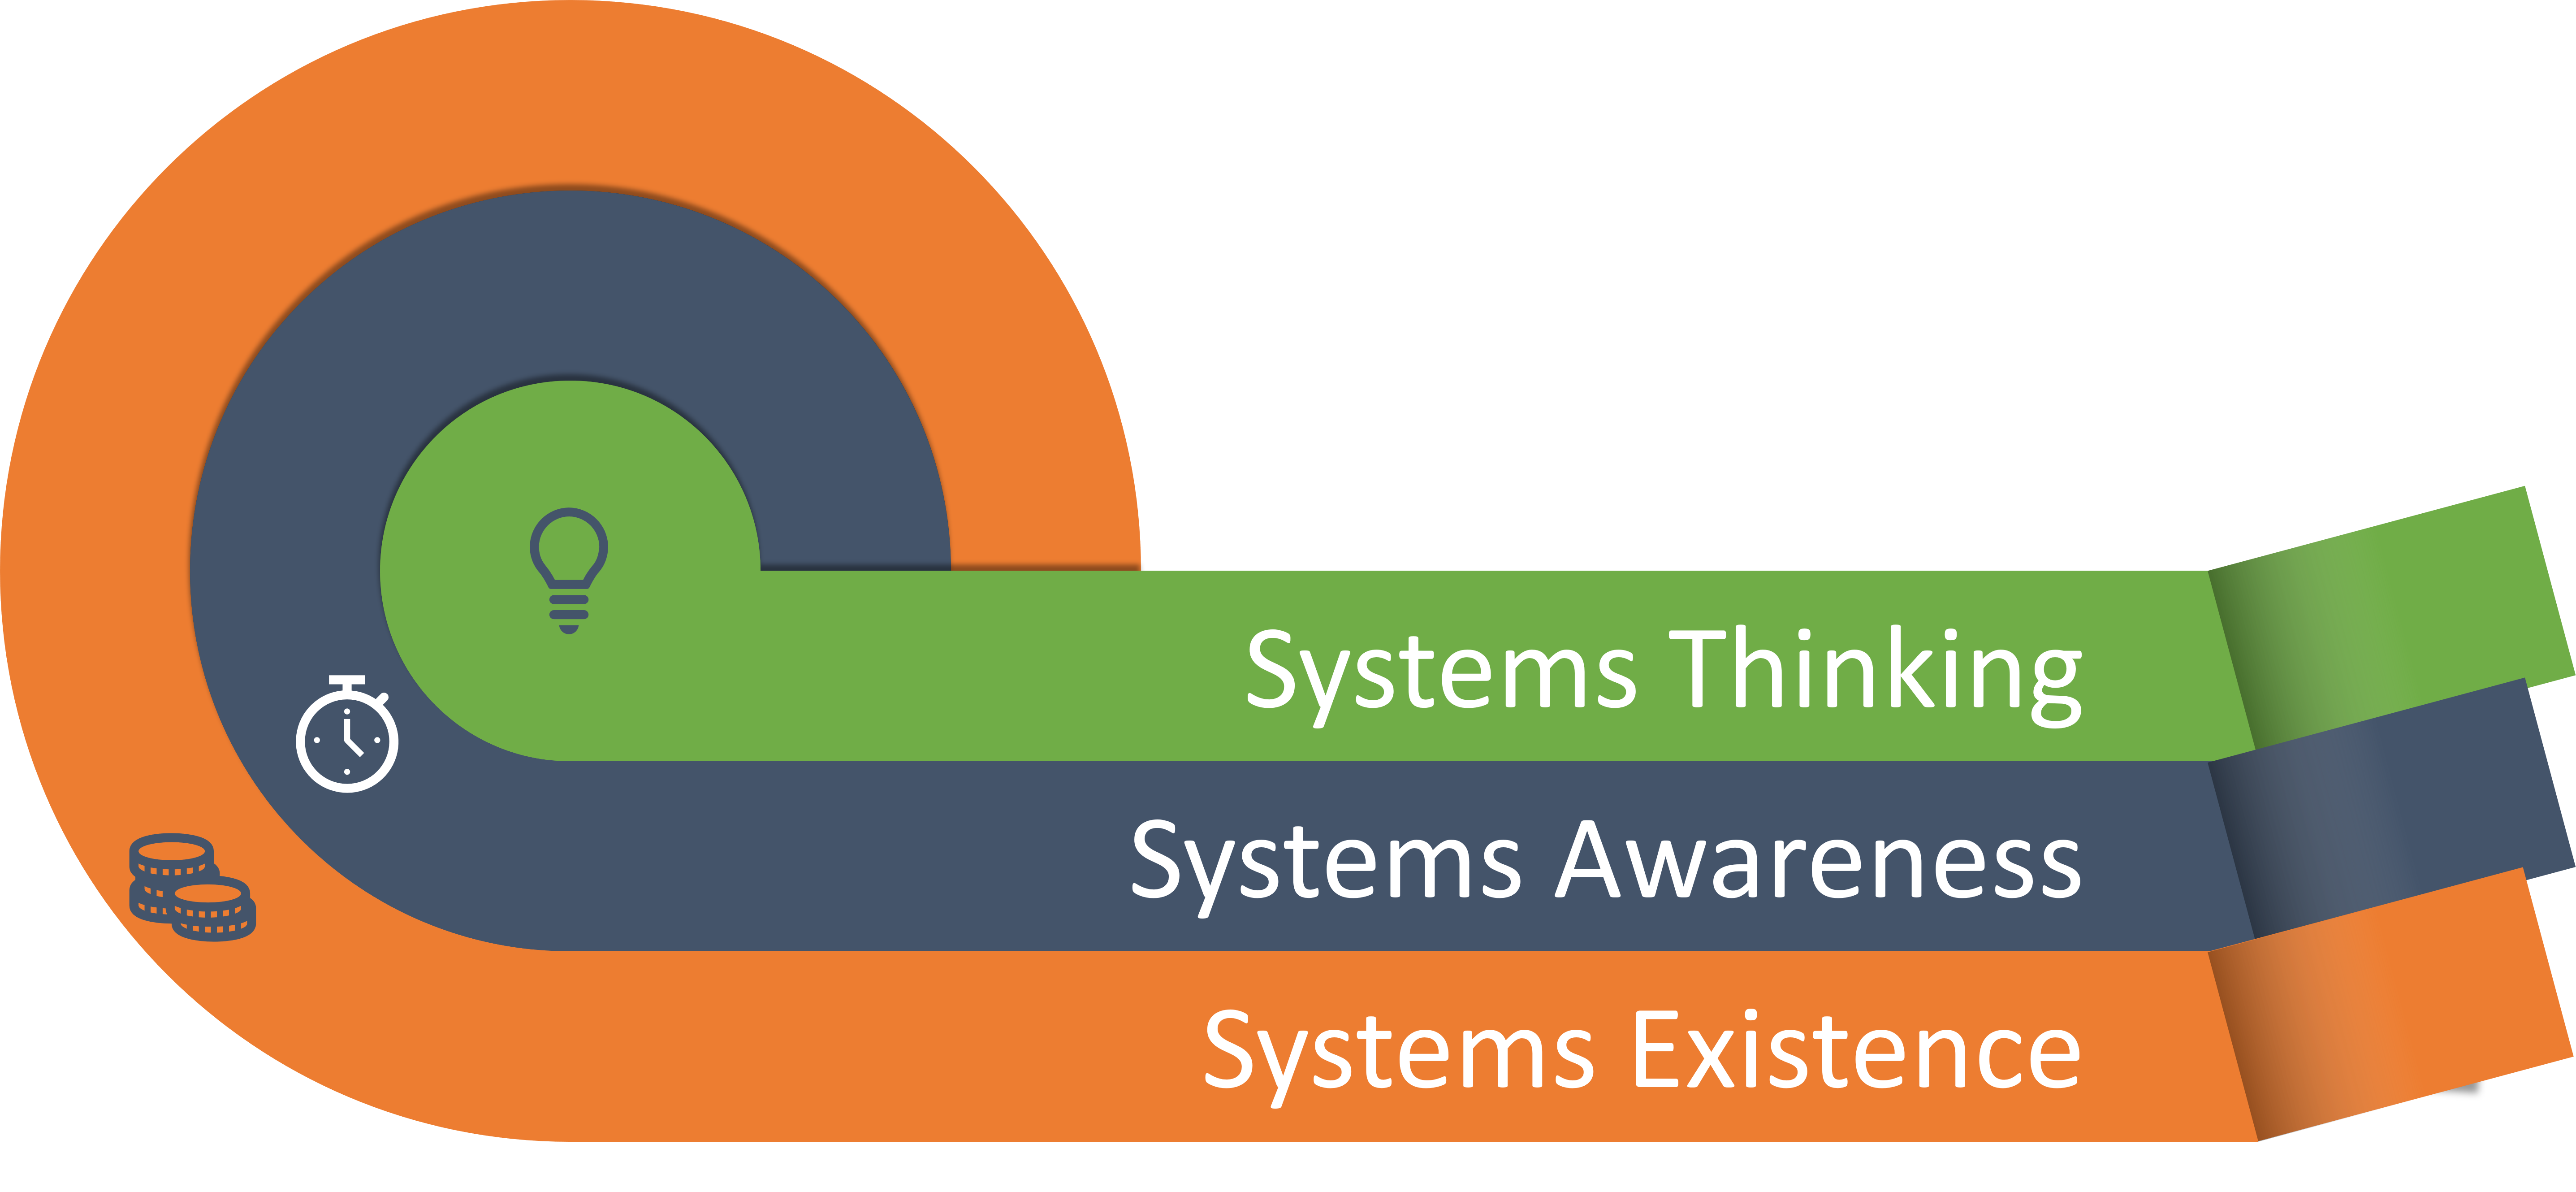
\includegraphics[width=0.9\textwidth]{systemsThinkingSnail.png}
\caption{Complete experimental setup (left) with close-up view of stage (right).}
\label{fig:systemsThinkingSnail}
\end{figure}

Figure 1.2 is conceptual in nature and self-explanatory. In science, it is argued that the only way to fully understand why a problem or element occurs and persists is to understand the parts in relation to the whole. [3] Standing in contrast to Descartes’s scientific reductionism and philosophical analysis, it proposes to view systems in a holistic manner. Consistent with systems philosophy, systems thinking concerns an understanding of a system by examining the linkages and interactions between the elements that compose the entirety of the system.

Science systems thinking attempts to illustrate that events are separated by distance and time and that small catalytic events can cause large changes in complex systems. Acknowledging that an improvement in one area of a system can adversely affect another area of the system, it promotes organizational communication at all levels to avoid the silo effect. Systems thinking techniques may be used to study any kind of system – natural, scientific, engineered, human or conceptual.

Systems thinking has been defined as an approach to problem solving, by viewing “problems” as parts of an overall system, rather than reacting to specific part, outcomes or events and potentially contributing to further development of unintended consequences. Systems thinking is not one thing but a set of habits or practices within a framework that is based on the belief that the component parts of a system can best be understood in the context of relationship with each other and with other systems, rather than in the isolation. Systems thinking focuses on cyclical rather than linear cause and effect.

\subsection{Think Globally, Act Locally}\index{Think Globally, Act Locally}

The approach adopted in this book is to recommend to globally conscious people and youth (especially STEM participants) to acquire an interest in the degree to which human designs act to modify the natural world.
\begin{enumerate}
\item More attention to design can alleviate problems revealed during operations because operational outcomes are inherent and linked to the physics of design
\item The on-line linking of individual designer’s decisions to evaluation at the system level and to stakeholder value is becoming more technically feasible. How?
\end{enumerate}

Define the system design space and partition it into the Functional domain, the Design Dependent Parameter domain, and the Optimization domain, etc.
Design Dependent Parameters (DDP’s) are suggested as the most overarching and most LINK between human designers and the human modified world. They established the design space and specific predicted and/or estimated values thereof drive design evaluation.
Design evaluation is the compass for stumbling through the design space in search of a modified world judged to be satisfactory by stakeholders.

	Add material by Kathia Laslo, PhD who directs Staybook University’s program in Leadership of Sustainable Systems . . . 
    
\subsection{Think About the End Before Beginning}\index{Think About the End Before Beginning}

From the thinking of Leonardo da Vinci
\begin{itemize}
\item WHY “To Make the World Better for People” (Retitle source here)
\item Human-made entities should be designed to satisfy human needs, wants, and objectives effectively, while minimizing system life-cycle cost as well as the intangible costs of ecological and societal impacts on the natural world
\item HOW ``Adopt and Practice Systems Thinking and Engineering''
\item A technologically based interdisciplinary process for bringing systems, products, structures, and services (human-made entities) into being
\end{itemize}

Reorient the Organization: Organization, humankind’s most important innovation, is the time-tested means for bringing human-made entities into being. While the main focus is nominally on the entities themselves, Systems Engineering embraces better strategy. Systems Engineering concentrates on what the entities do before determining what the entities are, with form following function. That is, instead of offering systems or system elements and products per se, the organizational focus should shift to designing, delivering, and sustaining functionality, a capability, or a solution.
\section{Relating Textbook STEA to STEM}\index{Relating Textbook STEA to STEM}
\section{Summary and Extensions}\index{Summary and Extensions}

Although this book focuses on the engineering of systems and on systems analysis, it would not have been intellectually prudent to begin the discussion at that level. Upon examination, it is evident that both the engineering and the analysis aspects of the focus are directed to systems. Accordingly, this chapter is devoted to helping the reader gain essential insight into systems in general, and systems thinking in particular, with orientation toward the engineering and analysis of technical systems.

System definitions, a discussion of system elements, and a high-level classification of systems provide an opening panorama. It is here that a consideration of the origin of systems provides an orientation to natural and human-made domains as an overarching dichotomy. The importance of this dichotomy cannot be overemphasized in the study and application of systems engineering and analysis. It is the suggested frame of reference for considering and understanding the interface and impact of the human-made world on the natural world and on humans. Individuals interested in obtaining an in-depth appreciation for this interface and the mitigation of environmental impacts are encouraged to read T. E. Graedel and B. R. Allenby, Industrial Ecology, 2nd ed., Prentice Hall, 2003. Also of contemporary interest is the issue of sustainability treated as part of an integrated approach to sustainable engineering by P. Stasinopoulos, M. H. Smith, K. Hargroves, and C. Desha, Whole System Design, Earthscan Publishing, 2009. These works are recommended as an extension to this chapter (as well as Chapter 16), because they illuminate and address the sensitive interface between the natural and the human-made.

This chapter is also anchored by the domains of systems science and systems engineering, beginning with the former and ending with the latter. Accordingly, it is important to recognize that at least one professional organization exists for each domain. For systems science, there is the International Society for the System Sciences (ISSS), originally named the “Society for General Systems Research.” ISSS was established at the 1956 meeting of the American Association for the Advancement of Science under the leadership of biologist Ludwig von Bertalanffy, economist Kenneth Boulding, mathematician–biologist Anatol Rapoport, neurophysiologist Ralph Gerard, psychologist James Miller, and anthropologist Margaret Mead.

The founders of the International Society for the System Sciences felt strongly that the systematic (holistic) aspect of reality was being overlooked or downgraded by the conventional disciplines, which emphasize specialization and reductionist approaches to science. They stressed the need for more general principles and theories and sought to create a professional organization that would transcend the tendency toward fragmentation in the scientific enterprise. The reader interested in exploring the field of systems science and learning more about the work of the International Society for System Sciences, may visit the ISSS website at

Most scientific and professional societies in the United States interact and collaborate with cognizant but independent honor societies. The cognizant honor society for systems engineering is the Omega Alpha Association (OAA), emerging under the motto “Think About the End Before the Beginning.” Chartered in 2006 as an international honor association, OAA has the overarching objective of advancing the systems engineering process and its professional practice in service to humankind. Among subordinate objectives are opportunities to (1) inculcate a greater appreciation within the engineering profession that every human design decision shapes the human-made world and determines its impact upon the natural world and upon people; (2) advance system design and development morphology through a better comprehension and adaptation of the da Vinci philosophy of thinking about the end before the beginning; that is, determining what designed entities are intended to do before specifying what the entities are and concentrating on the provision of functionality, capability, or a solution before designing the entities per se; and (3) encourage excellence in systems engineering education and research through collaboration with academic institutions and professional societies to evolve robust policies and procedures for recognizing superb academic programs and students. The OAA website, provides information about OAA goals and objectives, as well as the OAA vision for recognizing and advancing excellence in systems engineering, particularly in academia.

Upon completion of, the reader should have obtained essential insight into systems and systems thinking, with a focus on systems engineering and analysis. The system definitions, classifications, and concepts presented in this chapter are intended to impart a general understanding about the following:

\begin{enumerate}
\item System classifications, similarities, and dissimilarities
\item The fundamental distinction between natural and human-made systems
\item The elements of a system and the position of the system in the hierarchy of systems
\item The domain of systems science, with consideration of cybernetics, general systems theory, and systemology
\item Technology as the progenitor for the creation of technical systems, recognizing its impact on the natural world
\item The transition from the machine or industrial age to the Systems Age, with recognition of its impact upon people and society
\item System complexity and scope and the demands these factors make on engineering in the Systems Age
\item The range of contemporary definitions of systems engineering used within the profession.
\end{enumerate}

\section*{Resources for Further Exploration}
\begin{itemize}
\item \href{http://innovbfa.viabloga.com/files/Herbert_Simon___theories_of_bounded_rationality___1972.pdf}{Theories of Bounded Rationality by Herbert A. Simon}
\item \href{https://medium.com/disruptive-design/tools-for-systems-thinkers-the-6-fundamental-concepts-of-systems-thinking-379cdac3dc6a}{Tools of a Systems Thinker by Leyla Acaroglu}
\item \href{http://www.afscet.asso.fr/resSystemica/Crete02/Dyer.pdf}{Beyond Systems Design as we know it? by Gordon Dyer}
\end{itemize}

%%----------------------------------------------------------------------------------------
%	PROBLEMS
%%----------------------------------------------------------------------------------------

%% SEA CHAPTER 1 - SYSTEM SCIENCE AND ENGINEERING
% SEA Question Location in \label{sea-Chapter#-Problem#}
% ANSWERS NEED UPDATING
\begin{exercises}
    \begin{exercise}
    \label{sea-1-26}
        Describe how systems thinking differs from systems engineering.
        % What benefits could result from improving systems thinking in society?
    \end{exercise}
    \begin{solution}
        Human society is characterized by its culture. Each human culture manifests itself through the medium of technology. It takes more than a single step for society to transition from the past, to present and future technology states. A common societal response is often to make the transition and then to adopt a static pattern of behavior. A better response would be to continuously seek new but well-thought-out possibilities for advancement. Improvement in technological literacy embracing systems thinking should increase the population of individuals capable of participating in this desirable endeavor. \textbf{Reference:}
    \end{solution}
    
    \begin{exercise}
    \label{sea-1-1}
        For a system with which you are familiar, justify why it is a system according to the definition in \Cref{sec:sectors-comprising-our}.
        % Pick a system with which you are familiar and verify that it is indeed a system per the system definition given at the beginning of Section 1.1.
    \end{exercise}
    \begin{solution}
        A river system (Mississippi) is an assemblage of a watershed, tributaries, and river banks that conveys water from the continental U.S. to the Gulf of Mexico. A municipal transportation system (Chicago) is an assemblage of trains, buses, subways, etc. that transports people among many city locations. A system of organization and management (Matrix) is based on a morphology and procedure, coordinating both line and support functions. An automobile manufacturer is a combination of factories, organizations, dealerships, etc., that delivers automobiles and related support services. A home is an assemblage of land, structure, utilities, furnishings, and people that provides a supportive place to live for one or more families. \textbf{Reference:}
    \end{solution}
    
    \begin{exercise} 
    \label{sea-1-2}
        Describe the components, attributes, and relationships in the system you used in Problem \ref{sea-1-1}.
        % Name and identify the components, attributes, and relationships in the system you picked in Question 1.
    \end{exercise}
    \begin{solution}
        The major components of a home are listed in Answer 1 above. Attributes include acreage, terrain, square footage, utility capacities, styles of decorating and furnishing, personalities, and philosophies. Relationships include layout, allocation of space to people, and approaches to living together. \textbf{Reference:}
    \end{solution}
    
    \begin{exercise}
    \label{sea-1-3}
        Name any system which includes a material that transforms over the system's life cycle and identify its structural components, operating components, and flow components.
        % Pick a system that alters material and identify its structural components, operating components, and flow components.
    \end{exercise}
    \begin{solution}
        A chemica1 processing plant is composed of structural components (building, tanks, piping), operating components (pumps, valves, controls), and flow components (chemical constituents, energy, information). \textbf{Reference:}
    \end{solution}
    
    \begin{exercise} 
    \label{sea-1-4_5}
        Name any complex system and
        \begin{enumerate}[label=\alph*)]
            \item Define the hierarchy related to the system.
            \item Define the system boundaries.
        \end{enumerate}
        % Select a complex system and discuss it in terms of the hierarchy of systems.
        % Select a complex system and identify some different ways of establishing its boundaries.
    \end{exercise}
    \begin{solution}
        A dam system can be considered a complex system.
        \begin{enumerate}[label=\alph*)]
            \item todo
            \item The boundaries of a dam system can be limited to the physical dam. Alternatively, the human-modified river system, which now has a lake, can be considered a part of the dam system. The related road system, for which the dam now provides a bridge over the river, can be included. The region’s tourism service system, for which the dam system now provides an array of additional services, can be included. \textbf{Reference:}
        \end{enumerate}
    \end{solution}
    
    \begin{exercise} 
    \label{sea-1-6_7_8}
        Identify and contrast
        \begin{enumerate}[label=\alph*)]
            \item Physical versus conceptual systems.
            \item Static versus dynamic systems.
            \item Closed versus open systems.
        \end{enumerate}
        % Identify and contrast a physical and conceptual system.
        % Identify and contrast a static and a dynamic system.
        % Identify and contrast a closed and an open system.
    \end{exercise}
    \begin{solution}
        \begin{enumerate}[label=\alph*)]
            \item A physical system such as a watershed has components which manifest themselves in space and time, whereas a conceptual system such as a work breakdown structure has no physical manifestations. It is only a plan for action. Reference: Section 1.2.2 (pages 6-7).
            \item A static system such as a highway system may be contrasted with an airline system, which is a dynamic system. In the former, structure exists without activity whereas in the latter, structural components are combined with the activities of aircraft being loaded and unloaded, aircraft in flight, and controls which govern the entire operation. Reference: Section 1.2.3 (page 7).
            \item A cannon is an example of a closed system. When a cannon is fired, a one–to–one correspondence exists between the initial and final states. However, the defense contractor’s design and manufacturing organization that produced the cannon and associated projectile is an open system, with a dynamic interaction of system components. These system components must be reconfigured and adapted to cope with changing requirements. \textbf{Reference:}
        \end{enumerate}
    \end{solution}
    
    \begin{exercise} 
    \label{sea-1-15}
        For any system of the following types, name any system property
        \begin{enumerate}[label=\alph*)]
            \item Dynamic system.
            \item Steady-state system.
        \end{enumerate}
        % Give an example of a random dynamic system property and of a steady state dynamic system property.
    \end{exercise}
    \begin{solution}
        \textbf{Reference:}
    \end{solution}
    
    \begin{exercise} 
    \label{sea-1-9}
        For each of the following systems, define a unique system and describe it in terms of components, attributes, and relationships
        \begin{enumerate}[label=\alph*)]
            \item Natural system.
            \item Human-made system.
            \item Human-modified system.
        \end{enumerate}
        % Pick a natural system and describe it in terms of components, attributes, and relationships; repeat for a human-made system; repeat for a human-modified system.
    \end{exercise}
    \begin{solution}
        \begin{enumerate}[label=\alph*)]
            \item A watershed is a natural system made up of objects or components such as land, vegetation, and the watercourse; attributes such as the soil type, timber species, and the river width; and relationships such as the distribution of the attributes over the terrain. 
            \item A chemical processing plant is a human–made system with components described in Answer 3 above, attributes such as tank volume and pipe diameter, and relationships such as the flow rates and the yield of final product per energy unit utilized.
            \item A person with a pacemaker is a human-modified system with components of body parts and pacemaker parts, attributes such as body mass, diseases, attitudes, battery, controller, and electrodes, and relationships such as implantation location, rhythm, and signal strength. \textbf{Reference:}
        \end{enumerate}
    \end{solution}
    
    \begin{exercise} 
    \label{sea-1-10_11_12}
        For any Human-made system (including the system from \ref{sea-1-9})
        \begin{enumerate}[label=\alph*)]
            \item Identify the system's purpose(s) and potential metrics to present its value.
            \item Describe the system's state at any arbitrary time during operation, at least one system behavior, and an overview of the system's process.
            \item Name any two related components of the system, define the purpose of each component as it relates to the other, and the necessary attributes of the component pair such that they contribute to the purpose(s) of the entire system.
        \end{enumerate}
        % Identify the purpose(s) of the above human-made system and name some possible measures of worth.
        % For the above human-made system, describe its state at some point in time, describe one of its behaviors, and summarize its process.
        % For the above human-made system, name two components that have a relationship, identify what need each component fills for the other component, and describe how the attributes of these two components must be engineered so that the pair functions together effectively in contributing to the system’s purpose(s).
    \end{exercise}
    \begin{solution}
        \begin{enumerate}[label=\alph*)]
            \item The purposes of a chemical processing plant in a market economy are to produce one or more chemical products and possibly byproducts that can be sold at a profit while fulfilling obligations to stakeholders and the public. Measures of worth include production cost per unit volume, product quality, flexibility of product mix, benefits to stakeholders, and compatibility with society. \textbf{Reference:}
            \item During startup the state of a chemical processing plant is that pipes and vessels are filled to a certain location and empty after that location; pumps for vessels being filled are running and valves are open while other pumps are not running and valves are closed. A behavior is that when a vessel is filled, the control system turns off the pump (in a batch system) or reduces its speed (in a continuous system) and activates the next step in the process. The process is to start up, achieve the designated operational speed for each subsystem, continuously monitor the production results and make needed adjustments, and eventually shut down and clean out. \textbf{Reference:}
            \item A pump and the tank it fills have a relationship. The pump provides the material that the tank needs, while the tank provides a location where the pump can store the material it needs to deliver. The attributes of the pump must be engineered so that it can reliably move the material(s) the tank needs at an adequate rate for any given speed of overall system operation. The attributes of the tank must be engineered so that it can store the quantities of material the pump must deliver without corrosion or contamination. Thus the downstream components have the material they need to fulfill the plant’s production purpose without problems of quality or pollution. \textbf{Reference:} 
        \end{enumerate}
    \end{solution}
    
    \begin{exercise} 
    \label{sea-1-14}
        For any Human-modified system (including the system from \ref{sea-1-9}), name some positive and negative impact(s) of the modification to the natural system.
        % For a human-modified system, identify some of the ways in which the modified natural system could be degraded and some of the ways in which it could be improved.
    \end{exercise}
    \begin{solution}
        Human introduction of plant or animal species into regions where they do not naturally occur can provide the benefits of those species in the new regions, but the new species may become excessively dominant in those regions due to lack of natural enemies, crowding out or harming beneficial native species. \textbf{Reference:}
    \end{solution}
    
    \begin{exercise} 
    \label{sea-1-13}
        Give examples of each of the following
        \begin{enumerate}[label=\alph*)]
            \item First-order relationship.
            \item Second-order relationship.
            \item Redundance.
        \end{enumerate}
        % Give an example of a first-order relationship, a second-order relationship, and redundance.
    \end{exercise}
    \begin{solution}
        \begin{enumerate}[label=\alph*)]
            \item In a computer system, the power supply and system board have a first-order relationship because the system board must receive the reduced voltage produced by the power supply in order to function, and the power supply would be useless if there were no system board to perform and coordinate the computer functions. 
            \item The system board has a second-order relationship with a math coprocessor, or a video processor, or with video memory. The system board could perform the functions of these additional components, but the added components relieve the system board’s workload, thereby improving its performance.
            \item  A second power supply or a mirror image hard disk drive provide redundance, ensuring that the system board can continue receiving electrical power and the data storage function, thereby helping to assure continuation of the computer system function. \textbf{Reference:}
        \end{enumerate}
    \end{solution}
    
    \begin{exercise} 
    \label{sea-1-16}
        Name any system that operates at equilibrium and another system that degrades over time.
        % Give an example of a system that reaches equilibrium and of a system that disintegrates over time.
    \end{exercise}
    \begin{solution}
        A forest reaches equilibrium. A tree is in equilibrium until it dies, and then it disintegrates. \textbf{Reference:}
    \end{solution}
    
    \begin{exercise} 
    \label{sea-1-17}
        The United States government, for example, can be divided and described as three individual entities of the executive, legislative, and judicial branches. Create an argument for why a government of this structure should either be considered a single system or three systems.
        % Is a government with executive, legislative, and judicial branches three systems or a single system? Why?
    \end{exercise}
    \begin{solution}
        The government described is a single system because the branches thereof are functionally related. \textbf{Reference:}
    \end{solution}
    
    \begin{exercise} 
    \label{sea-1-19}
        Give any example of cybernetics and define why the example is appropriate.
        % Explain cybernetics by using an example of your choice.
    \end{exercise}
    \begin{solution}
        Cybernetics may be described and explained by considering the early mechanical version of a governor to control the revolutions per minute (RPM) of an engine. Centrifugal force, acting through a weight mechanism on the flywheel, is used to sense RPM. The outward movement of the weight against a spring acts through a link to decrease the throttle setting, thus reducing engine speed. \textbf{Reference:}
    \end{solution}
    
    \begin{exercise} 
    \label{sea-1-21}
        Do all systems at higher levels of Boulding's Hierarchy necessarily incorporate the lower levels of the hierarchy? If not, provide a specific system example.
        % Select a system at one of the higher levels in Boulding’s hierarchy and describe if it does or does not incorporate the lower levels.
    \end{exercise}
    \begin{solution}
        \textbf{Reference:}
    \end{solution}
    
    \begin{exercise} 
    \label{sea-1-22}
        Describe a novel system that may be necessary for society 50 to 100 years in the future and
        \begin{enumerate}[label=\alph*)]
            \item Define the system requirements.
            \item Define the system objectives.
        \end{enumerate}
        % Identify a societal need, define the requirements of a system that would fill that need, and define the objective(s) of that system.
    \end{exercise}
    \begin{solution}
        Efficient transportation system to the Moon and/or Mars. \textbf{Reference:}
    \end{solution}
    
    \begin{exercise} 
    \label{sea-1-25}
        For the system described in Question \ref{sea-1-22}
        \begin{enumerate}[label=\alph*)]
            \item Identify factors which led to the need for a new system.
            \item Identify other societal factors which may evolve in parallel and lead to other changes or innovations.
        \end{enumerate}
        % Name some of the factors driving technological advancement and change.
    \end{exercise}
    \begin{solution}
        \begin{enumerate}[label=\alph*)]
            \item Factors driving technological change include attempts to respond to unmet current needs and attempts to perform ongoing activities in a more efficient and effective manner, as well as social factors, political objectives, ecological concerns, and the desire for environmental sustainability. \textbf{Reference:}
            \item todo
        \end{enumerate}
    \end{solution}
    
    \begin{exercise} 
    \label{sea-1-23}
        Compare and contrast systemology and synthesis.
        % What are the similarities of systemology and synthesis?
    \end{exercise}
    \begin{solution}
        Both systemology and synthesis produce systems. Systemology produces a system of processes by which systems are brought into being and carried through the life cycle. Synthesis produces any kind of system. Synthesis is a part of systemology and also a product of systemology. \textbf{Reference:}
    \end{solution}
    
    \begin{exercise} 
    \label{sea-1-24}
        Classify a technical system.
        % What difficulty is encountered in attempting to classify technical systems?
    \end{exercise}
    \begin{solution}
        The phrase “technical system” is used to represent all types of human–made artifacts, including engineered products and processes. Classifying a technical system is generally difficult, because a technical system derives its inputs from several disciplines or fields which may be very different from one another. \textbf{Reference:}
    \end{solution}
    
    \begin{exercise} 
    \label{sea-1-27}
        Compare and contrast the attributes of the Machine (Industrial) Age and the Systems Age.
        % Identify the attributes of the Machine or Industrial Age and the Systems Age.
    \end{exercise}
    \begin{solution}
        Attributes of the Machine Age are determinism, reductionism, physical, cause and effect, and closed system thinking. The Systems Age has attributes of open systems thinking, expansionism, human–machine interfacing, automation, optimization, and goal orientation. \textbf{Reference:}
    \end{solution}
    
    \begin{exercise} 
    \label{sea-1-28}
        Identify key differences between synthetic and analytical thinking. Is one method of thinking always preferable? Why or why not?
        % Explain the difference between analytic and synthetic thinking.
    \end{exercise}
    \begin{solution}
        Analytic thinking seeks to explain the whole based on explanations of its parts. Synthetic thinking explains something in terms of its role in a larger context. \textbf{Reference:}
    \end{solution}
    
    \begin{exercise} 
    \label{sea-1-29}
        What challenges make the Systems Age unique from other periods of human evolution?
        % What are the special engineering requirements and challenges in the Systems Age?
    \end{exercise}
    \begin{solution}
        The special engineering requirements of the Systems Age are those which pertain to integration, synthesis, simulation, economic analysis, and environmental concerns, along with the necessity to bring the classical engineering disciplines to bear on the system under development through collaboration. \textbf{Reference:}
    \end{solution}
    
    \begin{exercise} 
    \label{sea-1-30}
        Compare and contrast systems engineering with other engineering disciplines.
        % What are the differences (and similarities) between systems engineering and the traditional engineering disciplines?
    \end{exercise}
    \begin{solution}
        Both systems engineering and the traditional engineering disciplines deal with technology and technical (human-made) entities. The focus of traditional engineering is on technical design of the entities in human-made systems, whereas systems engineering concentrates on what the entities are intended to do (functional design) before determining what the entities are. Traditional engineering focuses on technical performance measures, whereas systems engineering considers all requirements of the client, system owner, and/or the user group, as well as the effects on related systems. Traditional engineering focuses on designing products for their operational uses, whereas systems engineering considers all the life cycles of the systems that include its products. Traditional engineering tends to proceed from the bottom-up, whereas systems engineering favors a top-down approach. Traditional engineering favors analytic thinking while systems engineering favors synthetic thinking. Traditional engineering applies the skills of particular engineering disciplines to problems, whereas systems engineering defines problems before determining what disciplines are needed. Systems engineering provides methodologies that facilitate effective teamwork among not only the traditional engineering disciplines, but also among other technical as well as social disciplines. \textbf{Reference:}
    \end{solution}
    
    \begin{exercise} 
    \label{sea-1-32}
        Identify a system which required an interdisciplinary approach to develop \textit{or} to implement. What disciplines were required and why?
        % Give an example of a problem requiring an interdisciplinary approach and identify the needed disciplines.
    \end{exercise}
    \begin{solution}
        The problem of predicting the availability and amount of oil and natural gas from a certain geological region, which might be available to refineries and power plants in another region in future time periods, requires the disciplines of geology, petroleum engineering, regional planning, civil engineering, ecological science, transportation engineering, and economics. The validity of the prediction depends largely upon the proper utilization and interpretation of findings by the relevant disciplines and their domains of inquiry. \textbf{Reference:}
    \end{solution}
    
    \begin{exercise} 
    \label{sea-1-33}
        Identify an interdiscipline and the disciplines from which it was derived.
        % Name an interdiscipline and identify the disciplines from which it was drawn.
    \end{exercise}
    \begin{solution}
        Systems engineering is an interdiscipline (sometimes called a multidiscipline or transdiscipline) drawn mainly from the engineering disciplines, but also from mathematics, operations research, systemology, project management, and increasingly, other fields. \textbf{Reference:}
    \end{solution}
    
    \begin{exercise} 
    \label{sea-1-35_36_38}
        For the following organizations, summarize their mission statements
        \begin{enumerate}[label=\alph*)]
            \item \href{http://isss.org/}{International Society for the Systems Sciences}
            \item \href{https://www.incose.org/}{International Council on Systems Engineering}
            \item \href{https://omegalpha.org/}{Omega Alpha Association}
        \end{enumerate}
        % Go to the website for ISSS given in Section 1.7 and summarize the goal of the society.
        % Go to the website for INCOSE given in Section 1.7 and summarize the goals of the council.
        % Go to the website for OAA and compare this honor society with one that you are familiar with.
    \end{exercise}
    \begin{solution}
        \begin{enumerate}[label=\alph*)]
            \item Independent exercise. Visit http://isss.org/
            \item Independent exercise. Visit https://www.incose.org/
            \item Independent exercise. Visit https://omegalpha.org/
        \end{enumerate}
    \end{solution}
    
    \begin{exercise} 
    \label{sea-1-37}
        Explain how the goals of ISSS and INCOSE differ.
        % Contrast the goals of ISSS and INCOSE as given in Section 1.7 or on the web.
    \end{exercise}
    \begin{solution}
        Independent exercise. Refer to the solution of \ref{sea-1-35_36_38}.
    \end{solution}
\end{exercises}
% SKIPPED
% sea-1-18 Identify a system-of-systems whose analysis could yield insights not available by separately analyzing the individual systems of which it is composed.
% sea-1-20 Give a system example at any five of the levels in Boulding’s hierarchy.
% sea-1-31 Given the recommendations in Educating the Engineer of 2020, what should be added to the curriculum with which you are familiar?
% sea-1-34 Write your own (preferred) definition of systems engineering.

